\begin{figure}[!h]
\begin{center}
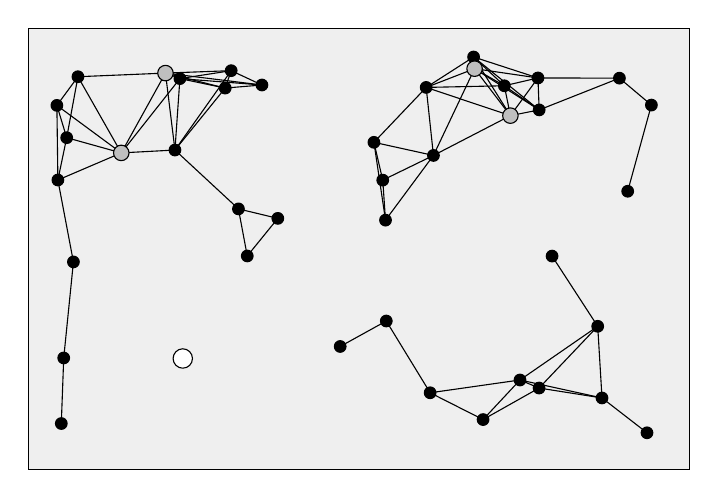
\begin{tikzpicture}[scale=1.4]
\fill[lightgray!25,draw=black] (0,0) rectangle (6,4);
\clip (0,0) rectangle (6,4);
\draw [](0.26,3.3) -- (0.269,2.623);
\draw [](0.26,3.3) -- (0.349,3.007);
\draw [](0.26,3.3) -- (0.451,3.56);
\draw [](0.26,3.3) -- (0.844,2.869);
\draw [](0.269,2.623) -- (0.349,3.007);
\draw [](0.269,2.623) -- (0.41,1.88);
\draw [](0.269,2.623) -- (0.844,2.869);
\draw [](0.3,0.414) -- (0.322,1.009);
\draw [](0.322,1.009) -- (0.41,1.88);
\draw [](0.349,3.007) -- (0.451,3.56);
\draw [](0.349,3.007) -- (0.844,2.869);
\draw [](0.451,3.56) -- (0.844,2.869);
\draw [](0.451,3.56) -- (1.245,3.593);
\draw [](0.844,2.869) -- (1.245,3.593);
\draw [](0.844,2.869) -- (1.331,2.895);
\draw [](0.844,2.869) -- (1.376,3.543);
\draw [](1.245,3.593) -- (1.331,2.895);
\draw [](1.245,3.593) -- (1.376,3.543);
\draw [](1.245,3.593) -- (1.787,3.457);
\draw [](1.245,3.593) -- (1.841,3.615);
\draw [](1.245,3.593) -- (2.12,3.485);
\draw [](1.331,2.895) -- (1.376,3.543);
\draw [](1.331,2.895) -- (1.787,3.457);
\draw [](1.331,2.895) -- (1.841,3.615);
\draw [](1.331,2.895) -- (1.907,2.361);
\draw [](1.376,3.543) -- (1.787,3.457);
\draw [](1.376,3.543) -- (1.841,3.615);
\draw [](1.376,3.543) -- (2.12,3.485);
\draw [](1.787,3.457) -- (1.841,3.615);
\draw [](1.787,3.457) -- (2.12,3.485);
\draw [](1.841,3.615) -- (2.12,3.485);
\draw [](1.907,2.361) -- (1.987,1.934);
\draw [](1.907,2.361) -- (2.264,2.275);
\draw [](1.987,1.934) -- (2.264,2.275);
\draw [](2.83,1.113) -- (3.248,1.344);
\draw [](3.136,2.965) -- (3.216,2.622);
\draw [](3.136,2.965) -- (3.241,2.259);
\draw [](3.136,2.965) -- (3.61,3.463);
\draw [](3.136,2.965) -- (3.676,2.846);
\draw [](3.216,2.622) -- (3.241,2.259);
\draw [](3.216,2.622) -- (3.676,2.846);
\draw [](3.241,2.259) -- (3.676,2.846);
\draw [](3.248,1.344) -- (3.646,0.693);
\draw [](3.61,3.463) -- (3.676,2.846);
\draw [](3.61,3.463) -- (4.04,3.739);
\draw [](3.61,3.463) -- (4.049,3.633);
\draw [](3.61,3.463) -- (4.319,3.478);
\draw [](3.61,3.463) -- (4.374,3.207);
\draw [](3.646,0.693) -- (4.126,0.45);
\draw [](3.646,0.693) -- (4.461,0.809);
\draw [](3.676,2.846) -- (4.049,3.633);
\draw [](3.676,2.846) -- (4.374,3.207);
\draw [](4.04,3.739) -- (4.049,3.633);
\draw [](4.04,3.739) -- (4.319,3.478);
\draw [](4.04,3.739) -- (4.374,3.207);
\draw [](4.04,3.739) -- (4.624,3.549);
\draw [](4.04,3.739) -- (4.635,3.259);
\draw [](4.049,3.633) -- (4.319,3.478);
\draw [](4.049,3.633) -- (4.374,3.207);
\draw [](4.049,3.633) -- (4.624,3.549);
\draw [](4.049,3.633) -- (4.635,3.259);
\draw [](4.126,0.45) -- (4.461,0.809);
\draw [](4.126,0.45) -- (4.634,0.736);
\draw [](4.319,3.478) -- (4.374,3.207);
\draw [](4.319,3.478) -- (4.624,3.549);
\draw [](4.319,3.478) -- (4.635,3.259);
\draw [](4.374,3.207) -- (4.624,3.549);
\draw [](4.374,3.207) -- (4.635,3.259);
\draw [](4.461,0.809) -- (4.634,0.736);
\draw [](4.461,0.809) -- (5.166,1.296);
\draw [](4.461,0.809) -- (5.205,0.646);
\draw [](4.624,3.549) -- (4.635,3.259);
\draw [](4.624,3.549) -- (5.363,3.547);
\draw [](4.634,0.736) -- (5.166,1.296);
\draw [](4.634,0.736) -- (5.205,0.646);
\draw [](4.635,3.259) -- (5.363,3.547);
\draw [](4.752,1.933) -- (5.166,1.296);
\draw [](5.166,1.296) -- (5.205,0.646);
\draw [](5.205,0.646) -- (5.613,0.33);
\draw [](5.363,3.547) -- (5.653,3.303);
\draw [](5.438,2.521) -- (5.653,3.303);
\fill [black,draw=black] (0.26,3.3) circle (1.5pt);
\fill [black,draw=black] (0.269,2.623) circle (1.5pt);
\fill [black,draw=black] (0.3,0.414) circle (1.5pt);
\fill [black,draw=black] (0.322,1.009) circle (1.5pt);
\fill [black,draw=black] (0.349,3.007) circle (1.5pt);
\fill [black,draw=black] (0.41,1.88) circle (1.5pt);
\fill [black,draw=black] (0.451,3.56) circle (1.5pt);
\fill [black,draw=black] (0.844,2.869) circle (1.5pt);
\fill [black,draw=black] (1.245,3.593) circle (1.5pt);
\fill [black,draw=black] (1.331,2.895) circle (1.5pt);
\fill [black,draw=black] (1.376,3.543) circle (1.5pt);
\fill [black,draw=black] (1.787,3.457) circle (1.5pt);
\fill [black,draw=black] (1.841,3.615) circle (1.5pt);
\fill [black,draw=black] (1.907,2.361) circle (1.5pt);
\fill [black,draw=black] (1.987,1.934) circle (1.5pt);
\fill [black,draw=black] (2.12,3.485) circle (1.5pt);
\fill [black,draw=black] (2.264,2.275) circle (1.5pt);
\fill [black,draw=black] (2.83,1.113) circle (1.5pt);
\fill [black,draw=black] (3.136,2.965) circle (1.5pt);
\fill [black,draw=black] (3.216,2.622) circle (1.5pt);
\fill [black,draw=black] (3.241,2.259) circle (1.5pt);
\fill [black,draw=black] (3.248,1.344) circle (1.5pt);
\fill [black,draw=black] (3.61,3.463) circle (1.5pt);
\fill [black,draw=black] (3.646,0.693) circle (1.5pt);
\fill [black,draw=black] (3.676,2.846) circle (1.5pt);
\fill [black,draw=black] (4.04,3.739) circle (1.5pt);
\fill [black,draw=black] (4.049,3.633) circle (1.5pt);
\fill [black,draw=black] (4.126,0.45) circle (1.5pt);
\fill [black,draw=black] (4.319,3.478) circle (1.5pt);
\fill [black,draw=black] (4.374,3.207) circle (1.5pt);
\fill [black,draw=black] (4.461,0.809) circle (1.5pt);
\fill [black,draw=black] (4.624,3.549) circle (1.5pt);
\fill [black,draw=black] (4.634,0.736) circle (1.5pt);
\fill [black,draw=black] (4.635,3.259) circle (1.5pt);
\fill [black,draw=black] (4.752,1.933) circle (1.5pt);
\fill [black,draw=black] (5.166,1.296) circle (1.5pt);
\fill [black,draw=black] (5.205,0.646) circle (1.5pt);
\fill [black,draw=black] (5.363,3.547) circle (1.5pt);
\fill [black,draw=black] (5.438,2.521) circle (1.5pt);
\fill [black,draw=black] (5.613,0.33) circle (1.5pt);
\fill [black,draw=black] (5.653,3.303) circle (1.5pt);

\fill [lightgray,draw=black] (0.844,2.869) circle (2pt);
%\node [red] at (0.844,2.869) {\tiny $7$};
\fill [lightgray,draw=black] (1.245,3.593) circle (2pt);
%\node [red] at (1.245,3.593) {\tiny $7$};
\fill [lightgray,draw=black] (4.049,3.633) circle (2pt);
%\node [red] at (4.049,3.633) {\tiny $7$};
\fill [lightgray,draw=black] (4.374,3.207) circle (2pt);
%\node [red] at (4.374,3.207) {\tiny $7$};
\fill [white,draw=black] (1.402,1.004) circle (2.5pt);
\end{tikzpicture}

\end{center}
\caption[Illustration of the state of the proximity graph after the first iteration.]{Illustration of the state of the proximity graph after the first iteration. Any of the gray points is to be removed in the next iteration, as they have the largest amount of neighbours.}
\label{fig:aa2}
\end{figure}
